\chapter{Bottom Up (Farina)}
Ricostruire, se $w \in L(G)$, una rightmost derivation al contrario
%%%%%%%%%%%%%%%%%%%%%%%%%%%%%%%%%%%%%%%%%%%%%%%%%%%%%%%%%%%%%%%%%%%%%%%%%%%%%%%%%%%%%%%%%%%%%%%%%%
\subsection{Esempio}
$S \rightarrow aABe$\\
$A \rightarrow Abc|b$\\
$B \rightarrow d$\\

w = abbcde visto che \'e rightmost devo espandere B dato che \'e il non terminale pi\'u a destra.
$S \rightarrow aABe \rightarrow aAde \rightarrow aAbcde \rightarrow abbcde $\\

\begin{center}
    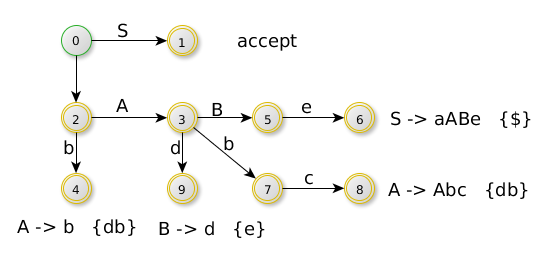
\includegraphics[scale=0.6]{Chapters/Img/c02_14.png}\\
\end{center} 

La sottolineatura significa che se arrivo in questo stato e sto leggendo come prossimo input una d o una b posso fare la riduzione della b usando A. Lo stesso vale per le altre, ovviamente con i loro simboli.
La roba fra parentesi graffe si chiama look-ahead set.

Nel grafo faccio quindi i seguenti passi (i numeri sono i nodi):
\begin{tabular}{ll}
    $0$   &   $abbcde\$$\\
    $0 \rightarrow 2$ consumando \lq $a$ \rq     &  $a || bbcde \$ $\\
    $2 \rightarrow 4$ consumando \lq $b$ \rq     &  $ab || bcde \$ $\\
    4 riduco $A \rightarrow b$  & $aA || bcde$\\
\end{tabular}
A questo punto torno al nodo 2 ovvero il precedente. Vado quindi in 3, perch\'e ho la A al posto della b che avevo prima.\\
torno a 2, vado in 3
\begin{tabular}{ll}
    $3 \rightarrow 7$ consumando \lq $b$ \rq     &  $aAb || cde \$ $\\
    $7 \rightarrow 8$ consumando \lq $c$ \rq     &  $aAbc || de \$ $\\
    8 riduco $A \rightarrow Abc$  & $aA || de$\\
    torno a 7, torno in 3, vado in 9 & \\
    $3 \rightarrow 9$ consumando \lq $d$ \rq     &  $aAd || e \$ $\\
    riduco $B \rightarrow d$ & $aAB || e \$ $\\
    torno a 3, vado in 5, vado in 6 & \\
    $5 \rightarrow 6$ consumando \lq $e$ \rq     &  $aABe || \$ $\\
    6 riduco $S \rightarrow aABe$ & $S || \$ $ \\
    torno a 0, vado in 1, ho finito & \\
\end{tabular}

Noi vogliamo avere grammatiche di tipo LALR(1). Grammatiche: $SLR(1) \subset LALR(1) \subset LR(1)$

\begin{center}
    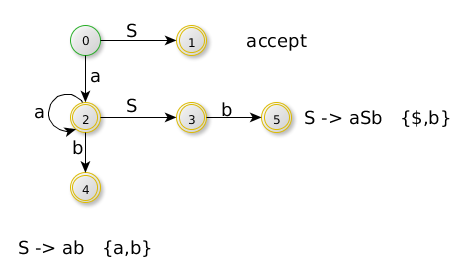
\includegraphics[scale=0.6]{Chapters/Img/c02_15.png}\\
\end{center} 

$S \rightarrow aSb | ab$\\
$w = aaabbb\$$

\begin{tabular}{ll}
    $0$                             &   $aaabbb\$$  \\ 
    $0 \rightarrow 2$               &   $a || aabbb\$$  \\ 
    $2 \rightarrow 2$               &   $aa || abbb\$$  \\ 
    $2 \rightarrow 2$               &   $aaa || bbb\$$  \\ 
    $2 \rightarrow 4$               &   $aaab || bb\$$  \\ 
    4 riduco $S \rightarrow ab$     &    $aaS || bb\$$  \\ 
    torno a 2, vado in 3, vado in 5 & \\
    $3 \rightarrow 5$               &   $aaSb || b\$$  \\ 
    5 riduco $S \rightarrow aSb$    &   $aS || b\$$  \\ 
    torno a 3, vado in 5            & \\
    $3 \rightarrow 5$               &   $aSb || \$$  \\ 
    5 riduco $S \rightarrow aSb$    &   $S || \$$  \\ 
    torno a 0, vado in 1, ho finito & \\
\end{tabular}\\[5pt]

Questa \'e una tabella:\\
\begin{tabular}{|l|l|l|}
    \hline
            &   terminali $\cup\ \$$                                     &   $V \backslash T$     \\
    \hline
    stati   &   shift-k: leggi un simbolo di input e vai allo stato     &   goto-k: descrive le funzioni di transizione  \\
            &   reduce $A \rightarrow b $                               &   identificate dai non terminali quando consumi roba\\
    \hline
\end{tabular}

\section{Algoritmo di shift/reduce}
(comune a SLR(1), LR(1), LALR(1))

\begin{tabular}{ll}
    input   &   w, tabella di parsing bottom-up di tipo $\diamond$, con $\diamond$ scelto fra $\{SLR(1), LALR(1), LR(1)\}$ G.\\
    output  &   derivazione rightmost di w se $w \in L(G)$, altrimenti error()\\  
\end{tabular}

\begin{lstlisting}
    stack.push(s_0);
    buffer = w$;
    while(true){
        let s = stack.top();
        if(M[s,b] == shift-k){
            stack.push(b);
            stack.push(k);
            let b = buffer.readNext(); 
        } else if(M[s,b] == "reduce A -> beta"){
            stack.pop() 2|beta| simboli;
            let j tale che M[m, A] = gj;
            push(A);
            push(j);
            output "A -> beta";
        } else if(M[s,b] = accetta){
            break;
        } else {
            error();
        }
    }
\end{lstlisting}

*sketo*
$S \rightarrow aSb | ab $

\begin{center}
    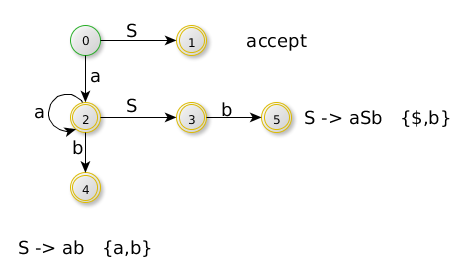
\includegraphics[scale=0.6]{Chapters/Img/c02_15.png}\\
\end{center} 

Questo \'e uguale ma scritto diversamente per separare $\{ \$, b\}$ in $\{4\}$ e $\{b\}$. Nel caso di $w=aaabbb\$$. Una caso rappresenta
il ramo pi\'u in alto, mentre l'altro il secondo ramo (pi\'u interno).

\begin{center}
    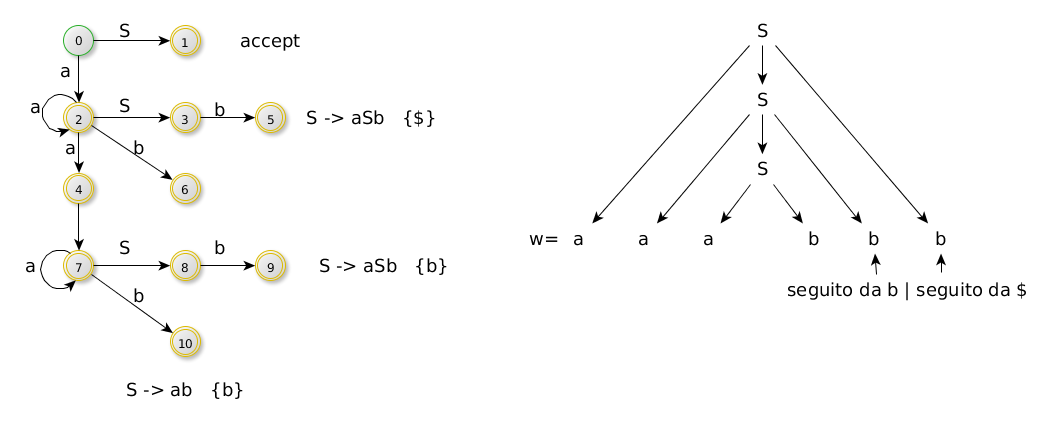
\includegraphics[scale=0.45]{Chapters/Img/c02_16.png}\\
\end{center} 

\begin{itemize}
    \item Automa caratteristico \\
    \item Lookahead Function \\
\end{itemize}

Coppie diverse di questi due insiemi ci danno tipi di grammatiche diverse.

Gli automi che stiamo utilizzando devono essere in grado di ricordare abbastanza da essere in grado di tornare indietro fino al punto 
in cui abbiamo sostituito una certa sequenza di terminali/non terminali con un'altra.

$G = (V,T,S,P)$, aggiungo una produzione $S' \rightarrow S \implies G' = (V \cup \{S'\},T,S',P \cup \{S' \rightarrow S\})$\\
\subsection{Closure}

All'inizio ho .S, ovvero non ho ancora letto nulla e devo leggere S.

All'inizio (il nodo iniziale), non ho ancora visto nulla. Visto che S pu\'o iniziare con aSb o ab non sappiamo davanti a quale sviluppo ci troviamo. Il primo stato \'e quindi 

$S' \rightarrow .S$\\
$S \rightarrow .aSb$\\
$S \rightarrow .ab$\\

Questo pu\'o essere visto come un nodo. Da questo stato mi muovo verso un altro stato (con una a-transizione, perch\'e vedo che iniziano 
quasi tutte con a). In questo stato avr\'o:
$S \rightarrow a.Sb$\\
$S \rightarrow a.b$\\

Adesso mi aspetto di vedere l'espansione di una S. Devo quindi aggiungere a questo nodo anche quelle produzioni, e diventa quindi:
$S \rightarrow a.Sb$\\
$S \rightarrow a.b$\\
$S \rightarrow .aSb$\\
$S \rightarrow .ab$\\

Quando computo uno stato ho i \textbf{kernel items} che poi vengono espansi con la \textbf{closure}.
Notare che gli ultimi due items sono gli stessi degli ultimi due del nodo precedente. 
Quella \'e la chiusura, mentre i primi due sono i generatori dello stato (kernel dello stato o \textbf{kernel items}).

Gli stati che terminali dell'automa (le foglie) sono del tipo $S \rightarrow ab.$ ,
quindi hanno incontrato tutto i simboli e possono essere ridotti (\textbf{reducing items}).

Dallo stato con 4 items che avevo prima, si pu\'o fare una b-transizione che va in uno di quelli stati terminali, ovvero:
$S \rightarrow ab.$\\
Questo perch\'e la seconda produzione si aspetta b, che poi completa quello che viene generato da quella produzione.
Sempre da quello stato con 4 produzioni partir\'a anche una a-transizione ed una S-transizione. Per vedere che transizioni devo avere, 
devo vedere la prima lettera dopo il punto per ogni item di quel nodo.

\section{Items}
$G=(V,T,S,P)$\\
$G'=(V \cup \{ S' \},T,S',P \cup \{S' \rightarrow S\})$, con $S' \not\in V$.

Un LR(0)-item di G' \'e una produzione di G con un punto in qualche posizione del body, ovvero $A \rightarrow \alpha . \beta$ .
Alla produzione della forma $A \rightarrow \varepsilon$ corrisponde un solo LR(0)-item, ovvero $A \rightarrow . $\\
L'item $A \rightarrow \alpha . \beta $ \'e detto:
\begin{tabular}{ll}
    iniziale    &   se $A = S' \land \alpha = \varepsilon \land \beta = S$, cio\'e se l'item \'e $S' \rightarrow .S$\\
    accepting   &   se $A = S' \land \alpha = S \land \beta = \varepsilon $, cio\'e se l'item \'e $S' \rightarrow S.$\\
    kernel      &   se \'e un iniziale o tale che $\alpha != \varepsilon$ \\
    closure     &   se $\alpha = \varepsilon$ e non \'e iniziale \\
    reducing    &   se non \'e accepting e $\beta = \varepsilon$, cio\'e se il punto \'e in fondo $\land !accepting$ \\
\end{tabular}


\chapter{Costruzione di un automa caratteristico LR(0) o LR(1)}
(data un'appropriata istanziazione di $P_0$ (stato iniziale) e closure function)

Prima di tutto facciamo la costruzione dell'automa caratteristico, usando l'algoritmo sotto riportato.

Istanziando $P_0$, closure otteniamo:
\begin{itemize}
	\item automi caratteristici LR(0)-automi $\leftarrow$ parsing SLR(1)\\
	\item automi caratteristici LR(1)-automi $\leftarrow$ parsing LR(1)\\
\end{itemize}
Lookahead function $LA:(FxP) \rightarrow p(T \cup \{ \$ \} )$
con F = insieme degli stati finali dell'automa caratteristico considerato. Si considerano stati finali gli stati che contengono almeno un reducing item.

L'automa caratteristico sar\'a necessario per la creazione della tabella di parsing.

\begin{lstlisting}
	Inizializzare la collezione Q di stati come {P_0};
	flag P_0 come non-marcato;

	while(ho uno stato non marcato P in Q){
		marca P;
		foreach(A -> a.Ybeta in P){
			tmp.add( A->aY.beta );
		}
		if(tmp == kernel(R)){ //per qualche R in Q
			tau(P, Y) = R; //goto function
		} else {
			newState = closure(tmp);
			tau(P, Y) = newState;
			Q.add(newState); //come non-marcato 
		}
	}
\end{lstlisting}

\subsection{Esempi di closure, grammatica SLR}
se ho la grammatica:\\
$S' \rightarrow S$\\
$S \rightarrow aSb|ab$\\
$closure_0(\{ S' \rightarrow .S\})$ \'e composta da:\\
$S \rightarrow .aSb$\\
$S \rightarrow .ab$\\

Se invece ho una grammatica:\\ 
$E' \rightarrow E$\\
$E \rightarrow E + T | T$\\
$T \rightarrow T * F | F$\\
$F \rightarrow (E) | id $\\

Allora $closure_0(\{ E' \rightarrow .E \})$ diventa \\
$E \rightarrow .E + T $ quelle con il punto prima della E le ho gi\'a aggiunte, non faccio nulla\\
$E \rightarrow .T $ ora aggiungo quelle con il punto prima della T\\
$T \rightarrow .T * F $ quelle con il punto prima della T le ho gi\'a aggiunte, non faccio nulla\\
$T \rightarrow .F $ ora aggiungo quelle con il punto prima della F\\
$F \rightarrow .(E)$ terminale dopo il punto, non devo aggiungere nulla\\
$F \rightarrow .id$ terminale dopo il punto, non devo aggiungere nulla\\
Si devono fare in ordine per non dimenticarsene in giro.

%%%%%%%%%%%%%%%%%%%%%%%%%%%%%%%%%%%%%%%%%%%%%%%%%%%%%%%%%%%%%%%%%%%%%%%%%%%%%%%%%%%%%%%%%%%%%%%%%%%%%%%%%%%%%%%%%%%%%%%%%%%%%%%%%%%%
\section{Algoritmo di $closure_0(P)$}
\begin{lstlisting}
	tag ogni item in P come non-marcato

	while(ho ancora un item I non marcato in P){
		marca I;
		if(I ha la forma A -> alpha .B beta){
			foreach ((B -> Y) in P){
				if(B -> Y not in P){
					add(B -> .Ya);
					segna P come non-marcato;
				}
			}
		}
	}
	return P;
\end{lstlisting}

\section{LR(0) automaton}
Si ricava utilizzando, nell'algoritmo di costruzione dell'automa caratteristico:
\begin{itemize}
	\item $P_0 = closure_0 ( \{ S' \rightarrow .S \} )$ per la grammatica G arricchita con $S' \rightarrow S$\\
	\item $ closure_0 $ per closure\\
\end{itemize}

%%%%%%%%%%%%%%%%%%%%%%%%%%%%%%%%%%%%%%%%%%%%%%%%%%%%%%%%%%%%%%%%%%%%%%%%%%%%%%%%%%%%%%%%%%%%%%%%%%%%%%%%%%%%%%%%%%%%%%%%%%%%%%%%%%%%
\subsection{Esempio}
$ S' \rightarrow S $\\
$ S \rightarrow aSb | ab $\\

\begin{tabular}{lll}
	$P_0=$ 	&	$S' \rightarrow .S$ 	& \\
			&	$S \rightarrow .aSb$ 	& \\
		 	&	$S \rightarrow .ab$ 	& \\
	$P_1=$ 	&	$S' \rightarrow S.$ 	& ci si arriva con una S-transizione (ACCEPT)\\
	$P_2=$ 	&	$S \rightarrow a.Sb$ 	& ci si arriva con una a-transizione\\
			&	$S \rightarrow a.b$ 	& \\
		 	&	$S \rightarrow .aSb$ 	& \\
		 	&	$S \rightarrow .ab$ 	& \\
		 	& 	$P_0 \text{ e } P_1$ sono finiti, guardo $P_2$ & \\
	$P_3=$ 	&	$S \rightarrow aS.b$ 	& ci si arriva con una S-transizione da $P_2$\\
	$P_4=$ 	&	$S \rightarrow ab.$ 	& ci si arriva con una b-transizione da $P_2$\\
	$P_5=$ 	&	$S \rightarrow .aSb$ 	& ci si arriva con una a-transizione da $P_2$ (stesse righe di $P_2$)\\
		 	&	$S \rightarrow .ab$ 	& la freccia quindi va da $P_2$ a $P_2$, perch\'e $P_5 \subset P_2$\\
		 	&	ora guardo $P_3$	& \\
	$P_6=$ 	&	$S \rightarrow aSb.$ 	& ci si arriva con una b-transizione da $P_3$\\
\end{tabular}  

%%%%%%%%%%%%%%%%%%%%%%%%%%%%%%%%%%%%%%%%%%%%%%%%%%%%%%%%%%%%%%%%%%%%%%%%%%%%%%%%%%%%%%%%%%%%%%%%%%%%%%%%%%%%%%%%%%%%%%%%%%%%%%%%%%%%
\section{Creazione della tabella di parsing}

\begin{tabular}{ll}
	$\tau$ 		&	funzione di transizione (GOTO) dell'automa caratteristico considerato.\\
	\textbf{LA} 	& 	lookahead function considerata.\\
\end{tabular}

La tabella di parsing bottom-up per la coppia prescelta di automa e lookahead function \'e una matrice 
$Q \otimes (V \cup \{ \$ \})$ dove Q \'e l'insieme degli stati dell'automa prescelto. \\[10pt]

$\forall$ entry (P,Y):
\begin{tabular}{ll}
	inserire \textbf{shift}					&	se $Y \in T \land \tau(P,Y) = R $\\
	inserire \textbf{reduce} $A \rightarrow \beta$   &	se $A \rightarrow \beta . \in P \land Y \in LA(P, A \rightarrow \beta) $\\
	inserire \textbf{accept()}				&	se $Y = \$ \land S' \rightarrow S. \in P $\\
	inserire \textbf{error()}				&	se $Y \in T \cup \{\$\} \land$ non \'e ancora stato inserito nulla\\
	applicando i passi precedenti 			& \\
	inserire \textbf{goto R}  				&	se $Y \in V\backslash T \land \tau (P,Y) = R $\\
\end{tabular}

%%%%%%%%%%%%%%%%%%%%%%%%%%%%%%%%%%%%%%%%%%%%%%%%%%%%%%%%%%%%%%%%%%%%%%%%%%%%%%%%%%%%%%%%%%%%%%%%%%%%%%%%%%%%%%%%%%%%%%%%%%%%%%%%%%%%
\subsection{Esercizio}
$SLR(1)$\\
$LR(0)$ automa \\
$LA(P, A \rightarrow \beta) = follow(A)\ \forall\ P \in Q$ (automa)\\



\begin{tabular}{|c|c|c|c|c|}
	\hline
	[numero nodo] 	&  [parte che & pu\'o avere & conflitti] & [goto part]\\
	\hline
		& 	\textbf{a} 	&	\textbf{b} 	& 	$\bm{\$}$ 	&	\textbf{S} 	\\
	\hline
	\textbf{0} 	&	S2	&		&			&	g1	\\
	\hline
	\textbf{1} 	&		&		&	ACCEPT	&		\\
	\hline
	\textbf{2} 	&	S2	&	S4	&			&	g3	\\
	\hline
	\textbf{3} 	&		&	s5	&			&		\\
	\hline
	\textbf{4} 	&		&	$R: S\rightarrow ab $	&	$R: S\rightarrow ab $		&		\\
	\hline
	\textbf{5} 	&		&	$R: S\rightarrow aSb $	&	$R: S\rightarrow aSb $		&		\\
	\hline
\end{tabular}

S = shift
R = reduce
g = goto

Se ho la parola $w = aabb\$$ faccio:
\begin{tabular}{|lll|}
	\hline
	0 			& 	$aabb\$$ 	& 	sono in 0 e vedo a. Faccio [0, a] nella tabella \\
	0a2			& 	$abb\$$ 	& 	sono in 2 e vedo a. Faccio [2, a] nella tabella \\
	0a2a2		& 	$bb\$$ 		& 	sono in 2 e vedo b. Faccio [2, b] nella tabella \\
	aa2a2b4 	& 	$b\$$ 		& 	sono in 4 e vedo b. Faccio il reduce (cella 4b) \\
				&				&	visto che crea 2S, e [2, S] = g3, aggiungo 3 	\\
	0a2S3		& 	$b\$$ 		& 	sono in 3 e vedo b. Faccio [3, b] nella tabella \\
	0a2S3b5		& 	$\$$ 		& 	sono in 5 e vedo $\$$. Faccio il reduce (cella 5$\$$ \\
				&				&	visto che crea 0S, e [0, S] = g1, aggiungo 1 	\\
	0S1			& 	$\$$ 		& 	ok perch\'e [S, 1] \'e accept 					\\
	\hline
\end{tabular}

\subsection{Esempio Conflitti Shift/Reduce}
(Esempio con una grammatica ambigua)\\

$E \rightarrow E + E | E * E | id $\\
automa LR(0)

\begin{center}
    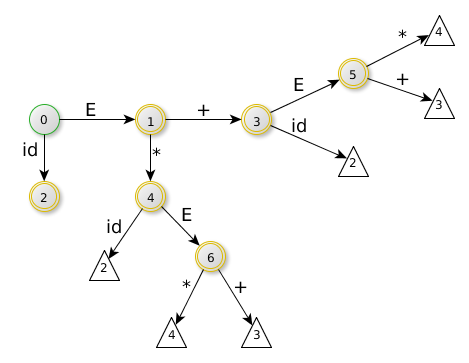
\includegraphics[scale=0.6]{Chapters/Img/c02_17.png}\\
\end{center} 

//Se va a triangoli, non parte dal kernel, altrimenti si(?)

0 =
\begin{tabular}{l}
	$E' \rightarrow .E$		\\
	$E \rightarrow .E + E$	\\
	$E \rightarrow .E * E$	\\
	$E \rightarrow .id$		\\
\end{tabular}\\[5pt]

1 =
\begin{tabular}{l}
	$E' \rightarrow E.$		\\
	$E \rightarrow E. + E$	\\
	$E \rightarrow E. * E$	\\
\end{tabular}\\[5pt]

2 =
\begin{tabular}{l}
	$E \rightarrow id.$		\\
\end{tabular}\\[5pt]

3 =
\begin{tabular}{l}
	$E \rightarrow E + .E$		\\
	$E \rightarrow .E * E$		\\
	$E \rightarrow .id $		\\
\end{tabular}\\[5pt]

4 =
\begin{tabular}{l}
	$E \rightarrow E * .E$		\\
	$E \rightarrow .E + E$		\\
	$E \rightarrow .E * E$		\\
	$E \rightarrow .id $		\\
\end{tabular}\\[5pt]

5 =
\begin{tabular}{l}
	$E \rightarrow E + E.$		\\
	$E \rightarrow E. + E$		\\
	$E \rightarrow E. * E$		\\
\end{tabular}\\[5pt]

6 =
\begin{tabular}{l}
	$E \rightarrow E * E.$		\\
	$E \rightarrow E. + E$		\\
	$E \rightarrow E. * E$		\\
\end{tabular}\\[5pt]

\begin{tabular}{|c|c|c|c|c|}
	\hline
		&	\textbf{id} 		&	$\bm{+}$	&	$\bm{*}$	&	$\bm{\$} $	\\
	\hline
	\textbf{0}	&	S2 		&		&		&			\\	
	\hline
	\textbf{1}	&	 		&	S3	&	S4	&	ACCEPT	\\	
	\hline
	\textbf{2}	&	 		&	$R:\ E \rightarrow id $		&	$R:\ E \rightarrow id $	& $R:\ E \rightarrow id $	\\	
	\hline
	\textbf{3}	&	S2 		&		&		&			\\	
	\hline
	\textbf{4}	&	S2 		&		&		&			\\	
	\hline
	\textbf{5}	&	 		&	$\bm{S3,\ R:\ E \rightarrow E+E}$	&	$\bm{S4,\ R:\ E \rightarrow E+E}$	&	$R:\ E \rightarrow E+E$		\\	
	\hline
	\textbf{6}	&	 		&	$\bm{S3,\ R:\ E \rightarrow E*E}$	&	$\bm{S4,\ R:\ E \rightarrow E*E}$	&	$R:\ E \rightarrow E*E$		\\	
	\hline
\end{tabular}\\[5pt]

\begin{tcolorbox}\begin{center}
	Visto che ci sono \textbf{conflitti} nella tabella, questa grammatica \textbf{non \'e SLR}. 
\end{center}\end{tcolorbox}

In questo caso i conflitti sono di tipo Shift/Reduce.
Ma possono essere anche di tipo Reduce/Reduce.

Tra le produzioni nelle celle colorate, quali sono quelle da tenere per avere una grammatica che associa a sinistra?

Nella cella [5, +] devo tenere R \lq\lq $E \rightarrow E + E $ \rq\rq\\
Nella cella [5, *] devo tenereS4 \\
Nella cella [6, +] devo tenere R \lq\lq $E \rightarrow E * E $ \rq\rq\\
Nella cella [6, *] devo tenere R \lq\lq $E \rightarrow E * E $ \rq\rq\\  

$W = id * id + id \$ $\\
$ 0 $\\
$ 0id2 $\\
$ 0E1 $\\
$ 0E1*4id2 $\\
$ 0E1*4E6 $\\
$ 0E1 $\\
$ 0E1+3id2 $\\
$ 0E1+3E5 $\\
$ 0E1 $\\
$ ok $\\

\Tree[.E [.E [.E id ] * [.E id ] ] + [.E id ] ]

\subsection{Esempio Conflitti Reduce/Reduce}
$S \rightarrow aAd | bBd | aBe | bAe$\\
$A \rightarrow c $\\
$B \rightarrow c $\\

Questa grammatica produce 4 stringhe, ogniuna in un modo, e quindi ovviamente non \'e ambigua.

\begin{center}
    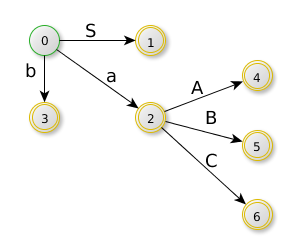
\includegraphics[scale=0.6]{Chapters/Img/c02_18.png}\\
\end{center} 

0 =
\begin{tabular}{l}
	$S' \rightarrow .S $		\\
	$S  \rightarrow .aAd $		\\
	$S  \rightarrow .bBd $		\\
	$S  \rightarrow .aBe $		\\
	$S  \rightarrow .bAe $		\\
\end{tabular}\\[5pt]

1 =
\begin{tabular}{l}
	$S' \rightarrow S. $		\\
\end{tabular}\\[5pt]

2 =
\begin{tabular}{l}
	$S \rightarrow a.Ad  $		\\
	$S  \rightarrow a.Be $		\\
	$A  \rightarrow .c $		\\
	$B  \rightarrow .c $		\\
\end{tabular}\\[5pt]

3 =
\begin{tabular}{l}
	$S \rightarrow b.Bd  $		\\
	$S  \rightarrow b.Ae $		\\
	$B  \rightarrow .c $		\\
	$A  \rightarrow .c $		\\
\end{tabular}\\[5pt]

4 =
\begin{tabular}{l}
	$S \rightarrow aA.d $		\\
\end{tabular}\\[5pt]

5 =
\begin{tabular}{l}
	$S \rightarrow aB.e $		\\
\end{tabular}\\[5pt]

6 =
\begin{tabular}{l}
	$A \rightarrow c. $		\\
	$B \rightarrow c. $		\\
\end{tabular}\\[5pt]

\begin{tabular}{|c|c|c|c|c|c|}
	\hline
		&	a 	& 	b 	&	d 	& 	e 	&	$\$$ 	\\
	\hline
	6	&	 	& 	& 	$R:\ A \rightarrow c $ 	&	$R:\ A \rightarrow c $ 	& 	\\	
		&	 	& 	& 	$R:\ B \rightarrow c $ 	&	$R:\ B \rightarrow c $ 	& 	\\	
	\hline
\end{tabular}

Anche se non \'e una grammatica ambigua ci sono multiple entries. Questo dipende dal modo in cui scegliamo i follow. 
Nel parsing canonico infatti non si usano gli item LR(0) ma gli item LR(1) perch\'e ci portiamo dietro informazione direttamente
dagli item. Questo riduce/rimuove i problemi di questo tipo.

Un item LR(1) canonico \'e del tipo $A \rightarrow \alpha . \beta, \delta$ con $\delta \subset T \cup \{ \$ \}$.\\

\section{LR(1)}
Negli automi caratteristici LR(1) si considera come stato iniziale lo stato che si ottiene facendo: 
$closure_1 (\{[ S' \rightarrow .S, \{ \$\}  ]\})$

\subsection{Esempio grammatica LR(1)}
$S \rightarrow aAd | aBe | bBd |bAe $\\
$A \rightarrow c$\\
$B \rightarrow c$\\


\begin{center}
    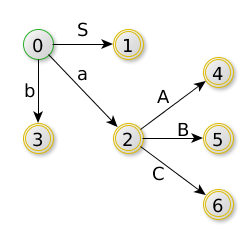
\includegraphics[scale=0.6]{Chapters/Img/c05_01.png}\\
\end{center}

0 =
\begin{tabular}{l}
	$S' \rightarrow .S,\ 	\{ \$ \} $		\\
	$S \rightarrow .aAd,\ 	\{ \$ \} $		\\
	$S \rightarrow .aBe,\ 	\{ \$ \} $		\\
	$S \rightarrow .bBd,\ 	\{ \$ \} $		\\
	$S \rightarrow .bAe,\ 	\{ \$ \} $		\\
\end{tabular}\\[5pt]

1 =
\begin{tabular}{l}
	$S' \rightarrow S.,\ 	\{ \$ \} $		\\
\end{tabular}\\[5pt]

2 =
\begin{tabular}{l}
	$S \rightarrow a.Ad,\ 	\{ \$ \} $		\\
	$S \rightarrow a.Be,\ 	\{ \$ \} $		\\
	$A \rightarrow .c,\ 	\{ d \} $		\\
	$B \rightarrow .c,\ 	\{ e \} $		\\
\end{tabular}\\[5pt]


3 =
\begin{tabular}{l}
	$S \rightarrow b.Bd,\ 	\{ ? \} $		\\
	$S \rightarrow b.Ae,\ 	\{ ? \} $		\\
	$A \rightarrow .c,\ 	\{ ?\} $		\\
	$B \rightarrow .c,\ 	\{ ?\} $		\\
\end{tabular}\\[5pt]


4 =
\begin{tabular}{l}
	$S \rightarrow aA.d,\ 	\{ ? \} $		\\
\end{tabular}\\[5pt]

5 =
\begin{tabular}{l}
	$S \rightarrow aB.e,\ 	\{ ? \} $		\\
\end{tabular}\\[5pt]

6 =
\begin{tabular}{l}
	$A \rightarrow c.,\ 	\{ d \} $		\\
	$B \rightarrow c.,\ 	\{ e \} $		\\
\end{tabular}\\[5pt]

\section{Algoritmo $Closure_1(P)$}
\begin{lstlisting}
	every item in P is unmarked
	while(exists an item I in P unmarked){
		mark I;
		if([ A -> alpha. B beta, delta ] in I){
			delta1 = Union(d in delta) first(beta d)
			foreach([ B -> Y ] in P){
				if([ B -> .Y ] not in proj(P)){ //projection is the first component of an item yet collected
					P.add([ B -> .Y, delta1] as unmarked)
				} else {
					if([ B -> .Y, gamma ] in P && delta1 not subset gamma ){
						update [ B -> .Y, gamma ] in [Bb -> .Y, gamma U delta1] as unmarked;
					}
				}
			}
		}
	}
	return P;
\end{lstlisting}

\section{Esempio grammatica LALR}

$S \rightarrow L = R | R$\\
$L \rightarrow *R|id$\\
$R \rightarrow L$\\

Computare la $closure_1( \{ [ S' \rightarrow S,\ \{\$\} ] \} )$ (nodo 0 e disegnare l'automa LR(1). Capire se \'e SLR(1)).

\begin{center}
    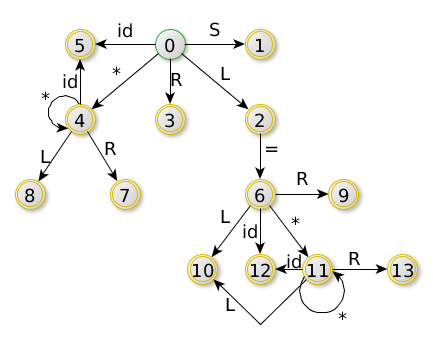
\includegraphics[scale=0.6]{Chapters/Img/c05_02.png}\\
\end{center}

0 =
\begin{tabular}{l}
	$S' \rightarrow .S,\ 	\{ \$ \} $		\\
	$S \rightarrow .L = R,\ 	\{ \$ \} $		\\
	$S \rightarrow .R,\ 	\{ \$ \} $		\\
	$L \rightarrow .*R,\ 	\{ \$ \} $		\\
	$L \rightarrow .id,\ 	\{ \$ \} $		\\
	$R \rightarrow .L,\ 	\{ \$ \} $		\\
\end{tabular}\\[5pt]

1 =
\begin{tabular}{l}
	$S' \rightarrow S.,\ 	\{ \$ \} $		\\
\end{tabular}\\[5pt]

2 =
\begin{tabular}{l}
	$S \rightarrow L.=R,\ 	\{ \$ \} $		\\
	$R \rightarrow L.,\ 	\{ \$ \} $		\\
\end{tabular}\\[5pt]

3 =
\begin{tabular}{l}
	$S \rightarrow R.,\ 	\{ \$ \} $		\\
\end{tabular}\\[5pt]

4 =
\begin{tabular}{l}
	$L \rightarrow *.R,\ 	\{ =, \$ \} $		\\
	$R \rightarrow .L,\ 	\{ =, \$ \} $		\\
	$L \rightarrow .id,\ 	\{ =, \$ \} $		\\
	$L \rightarrow .*R,\ 	\{ =, \$ \} $		\\
\end{tabular}\\[5pt]

5 =
\begin{tabular}{l}
	$L \rightarrow id.,\ 	\{ =, \$ \} $		\\
\end{tabular}\\[5pt]

6 =
\begin{tabular}{l}
	$S \rightarrow L = .R,\ 	\{ \$ \} $		\\
	$R \rightarrow .L,\ 	\{ \$ \} $		\\
	$L \rightarrow .*R,\ 	\{ \$ \} $		\\
	$L \rightarrow .id,\ 	\{ \$ \} $		\\
\end{tabular}\\[5pt]

7 =
\begin{tabular}{l}
	$L \rightarrow *R.,\ 	\{ =, \$ \} $		\\
\end{tabular}\\[5pt]

8 =
\begin{tabular}{l}
	$R \rightarrow L.,\ 	\{ =, \$ \} $		\\
\end{tabular}\\[5pt]

9 =
\begin{tabular}{l}
	$S \rightarrow L = R.,\ 	\{ \$ \} $		\\
\end{tabular}\\[5pt]

10 =
\begin{tabular}{l}
	$R \rightarrow L.,\ 	\{ \$ \} $		\\
\end{tabular}\\[5pt]

11 =
\begin{tabular}{l}
	$L \rightarrow *.R,\ 	\{ \$ \} $		\\
	$R \rightarrow .L,\ 	\{ \$ \} $		\\
	$L \rightarrow .*R,\ 	\{ \$ \} $		\\
	$L \rightarrow .id,\ 	\{ \$ \} $		\\
\end{tabular}\\[5pt]

12 =
\begin{tabular}{l}
	$L \rightarrow id.,\ 	\{ \$ \} $		\\
\end{tabular}\\[5pt]

13 =
\begin{tabular}{l}
	$L \rightarrow *R.,\ 	\{ \$ \} $		\\
\end{tabular}\\[5pt]

Notare che i nodi 8 e 10 sembrano uguali ma non lo sono perch\'e hanno lookahead diversi; anche nel gravo saranno nodi distinti 
mentre se avessimo fatto un automa LR(0) sarebbero stati uniti. Lo stesso automa LR(0):

\begin{center}
    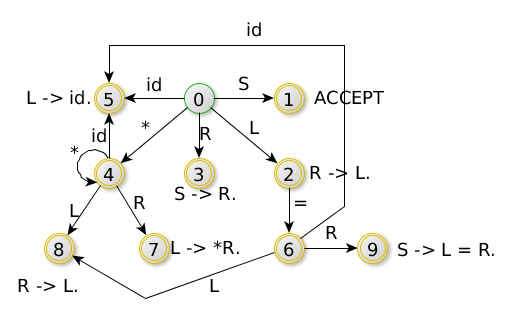
\includegraphics[scale=0.6]{Chapters/Img/c05_03.png}\\
\end{center}

Quest'ultimo automa ha almeno uno shift/reduce conflict mentre l'automa LR(1) non ne avr\'a.

Guardiamo se \'e SLR(1) 

\begin{tabular}{|c|c|c|c|c|c|c|c|}
	\hline
		&	\textbf{id} 	& $\bm{*}$	& $\bm{*}$	& $\bm{*}$	& 	\textbf{S}  & \textbf{L} & \textbf{R} \\  
	\hline
	\textbf{0}	&	S5 	& S4 	& 		& 		& 1 	& 2 	& 3 	\\
	\hline
	\textbf{1}	&		& 		& 		& ACC 	& 		& 		& 		\\
	\hline
	\textbf{2}	&		& 		& S6 	& r: $R \rightarrow L$ & 	& 	 	& 		\\
	\hline
	\textbf{3}	&		& 		& 		& r: $S \rightarrow R$ & 	& 		& 		\\
	\hline
	\textbf{4}	&	S5 & S4 	& 		& 						&	& 8 	& 7		\\
	\hline
	\textbf{5}	&		&		& r: $L \rightarrow id$ & r: $L \rightarrow id$ & 	&	&	\\
	\hline
	\textbf{6}	&	S12 & S11 	& 		& 						&	& 10 	& 9		\\	
	\hline
	\textbf{7}	&		&		& r: $L \rightarrow *R$ & r: $L \rightarrow *R$ & 	&	&	\\
	\hline
	\textbf{8}	&		&		& r: $R \rightarrow L$ & r: $R \rightarrow L$  & 	&	&	\\	
	\hline
	\textbf{9}	&		& 		& 		& r: $S \rightarrow L = R$ & 	& 		& 		\\	
	\hline
	\textbf{10}	&		& 		& 		& r: $R \rightarrow L$ & 	& 		& 		\\	
	\hline
	\textbf{11}	&	S12 & S11 	& 		& 						&	& 10 	& 13		\\		
	\hline
	\textbf{12}	&		& 		& 		& r: $L \rightarrow id$ & 	& 		& 		\\		
	\hline
	\textbf{13}	&		& 		& 		& r: $L \rightarrow *R$ & 	& 		& 		\\		
	\hline
\end{tabular}

visto che non ci sono conglitti questa grammatica \'e LR(1).
Gli stati 4 e 11 hanno la stessa proiezione; possiamo quindi fare: 
$P_1 \cup P_2\quad A \rightarrow \alpha . \beta,\ \delta_1 \cup \delta_2$.

Lo posso fare per 4 e 11, 5 e 12, 8 e 10, 7 e 13

\begin{tabular}{|c|c|c|c|c|c|c|c|}
	\hline
		&	\textbf{id} 	& $\bm{*}$	& $\bm{*}$	& $\bm{*}$	& 	\textbf{S}  & \textbf{L} & \textbf{R} \\  
	\hline
	\textbf{411}	&	S512 & S411 	& 		& 		& 810 	& 2 	& 713 	\\
	\hline
	\textbf{512}	&		& 		& r: $L \rightarrow id$		& r: $L \rightarrow id$ 	& 		& 		& 		\\
	\hline
	\textbf{713}	&		& 		& r: $L \rightarrow *R$ 	& r: $L \rightarrow *R$		& 		& 	 	& 		\\
	\hline
	\textbf{810}	&		& 		& r: $r \rightarrow L$ 	& r: $R \rightarrow L$		& 		& 	 	& 		\\
	\hline
\end{tabular}

Dovr\'o anche aggiornare i vari shift e goto delle altre righe per farli andare ai nodi nuovi. S5 ed S12 diventeranno S512.

La grammatica cos'\i generata \'e LALR perch\'e nella tabella non ci sono conflitti.

\subsection{Ricorda}
$ SLR(1) \subset LALR(1) \subset LR(1)$

Grammatica SLR(1)\\
$E' \rightarrow E$\\
$E \rightarrow E + T | T$\\
$T \rightarrow T * F | F$\\
$F \rightarrow (E) | id $\\

Grammatica LR(1)\\
$S \rightarrow aAd | aBe | bBd |bAe $\\
$A \rightarrow c$\\
$B \rightarrow c$\\

Grammatica LALR\\
$S \rightarrow L = R | R$\\
$L \rightarrow *R|id$\\
$R \rightarrow L$\\

\section{Algoritmo LALR(1) (inefficiente)}
\begin{itemize}
	\item[1.] 	Costruzione di $A_1$ (LR(1) automaton) \\
	\item[2.] 	Creo LR(1) Merged Automa $A_2$ (mergio gli stati che hanno la stessa proiezione). 
				Se lo stato $P \in A_2$ e'' il merging di $Q_1, ..., Q_k$ di $A_1$ e $Q_1$ ha una Y-transizione a $Q'_1$ allora 
				P ha una Y-transizione allo stato $P' \ / \ proj(P') = proj(Q') $\\
	\item[3.] 	$\forall\ P$ finale, $\forall\ [ A \rightarrow \beta.,\ \delta_i] \in P\ 
				LA(P, A \rightarrow \beta) = \cup_{\delta_i} [A \rightarrow \beta .,\ \delta _i] \in P$\\
\end{itemize}

\subsection{Esempio (Vedi esempio conflitti reduce/reduce)}
$S \rightarrow aAd | aBe | bBd | bAe$\\
$A \rightarrow c$\\
$B \rightarrow c$\\

Faccio LR(1) automa 

\begin{center}
    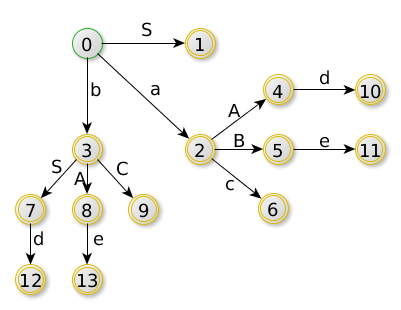
\includegraphics[scale=0.6]{Chapters/Img/c05_04.png}\\
\end{center}

0 =
\begin{tabular}{l}
	$S' \rightarrow .S,\  \{ \$ \}$		\\
	$S  \rightarrow .aAd,\  \{ \$ \}$	\\
	$S  \rightarrow .bBd,\  \{ \$ \}$	\\
	$S  \rightarrow .aBe,\  \{ \$ \}$	\\
	$S  \rightarrow .bAe,\  \{ \$ \}$	\\
\end{tabular}\\[5pt]

1 =
\begin{tabular}{l}
	$S' \rightarrow S.,\  \{ \$ \}$		\\
\end{tabular}\\[5pt]

2 =
\begin{tabular}{l}
	$S \rightarrow a.Ad  ,\  \{ \$ \}$	\\
	$S  \rightarrow a.Be ,\  \{ \$ \}$	\\
	$A  \rightarrow .c ,\  \{ d \}$	\\
	$B  \rightarrow .c ,\  \{ e \}$	\\
\end{tabular}\\[5pt]

3 =
\begin{tabular}{l}
	$S \rightarrow b.Bd  ,\  \{ \$ \}$	\\
	$S  \rightarrow b.Ae ,\  \{ \$ \}$	\\
	$B  \rightarrow .c ,\  \{ d \}$	\\
	$A  \rightarrow .c ,\  \{ e \}$	\\
\end{tabular}\\[5pt]

4 =
\begin{tabular}{l}
	$S \rightarrow aA.d ,\  \{ \$ \}$	\\
\end{tabular}\\[5pt]

5 =
\begin{tabular}{l}
	$S \rightarrow aB.e ,\  \{ \$ \}$	\\
\end{tabular}\\[5pt]

6 =
\begin{tabular}{l}
	$A \rightarrow c.,\  \{ d \}$	\\
	$B \rightarrow c.,\  \{ e \}$	\\
\end{tabular}\\[5pt]

7 =
\begin{tabular}{l}
	$S \rightarrow bB.d,\  \{ \$ \}$	\\
\end{tabular}\\[5pt]

8 =
\begin{tabular}{l}
	$S \rightarrow bA.e,\  \{ \$ \}$	\\
\end{tabular}\\[5pt]

9 =
\begin{tabular}{l}
	$B \rightarrow c.,\  \{ d \}$	\\
	$A \rightarrow c.,\  \{ e \}$	\\
\end{tabular}\\[5pt]

10 =
\begin{tabular}{l}
	$S \rightarrow aAd.,\  \{ \$ \}$	\\
\end{tabular}\\[5pt]

11 =
\begin{tabular}{l}
	$S \rightarrow aBe.,\  \{ \$ \}$	\\
\end{tabular}\\[5pt]

12 =
\begin{tabular}{l}
	$S \rightarrow bBd.,\  \{ \$ \}$	\\
\end{tabular}\\[5pt]

13 =
\begin{tabular}{l}
	$S \rightarrow bAe.,\  \{ \$ \}$	\\
\end{tabular}\\[5pt]

Gli stati 6 e 9 hanno la stessa proiezione quindi li mergio in \\

14 = 
\begin{tabular}{l}
	$A \rightarrow c.,\  \{ d \}$	\\
	$B \rightarrow c.,\  \{ e \}$	\\
	$A \rightarrow c.,\  \{ e \}$	\\
	$B \rightarrow c.,\  \{ d \}$	\\
\end{tabular}\\[5pt]

Sostituisco 14 a 6 e 9, faccio una transizione da 3 a 14

\begin{tabular}{|c|c|c|c|c|c|c|c|c|c|}
	\hline
		&	\textbf{a} 	& \textbf{b}	& \textbf{c}	& \textbf{d}	& \textbf{e} 	& $\bm{\$}$ & \textbf{S} & \textbf{A} & \textbf{B}	\\  
	\hline
	\textbf{0}	&	S2 	& S3 	& 		& 		&  	&  	& g1 &  & 	\\
	\hline
	\textbf{1}	&	 	&  	& 		& 		&  	&  ACC	&  &  & 	\\
	\hline
	\textbf{2}	&	 	&  	& 	S14	& 		&  	&  	&  &  g4  & g5	\\
	\hline
	\textbf{3}	&	 	&  	& 	S14	& 		&  	&  	&  &  g8  & g7	\\
	\hline
	\textbf{4}	&	 	&  	& 		& 	S10	&  	&  	&  &    & \\
	\hline
	\textbf{5}	&	 	&  	& 		& 		& S11  	&  	&  &    & 	\\
	\hline
	\textbf{7}	&	 	&  	& 		& 	S12	&   	&  	&  &   & 	\\
	\hline
	\textbf{8}	&	 	&  	& 		& 		& S13  	&  	&  &    & 	\\
	\hline
	\textbf{10}	&	 	&  	& 		& 		&   	& $S \rightarrow aAd$ 	&  &    & 	\\
	\hline
	\textbf{11}	&	 	&  	& 		& 		&   	& $S \rightarrow aBe$ 	&  &    & 	\\
	\hline
	\textbf{12}	&	 	&  	& 		& 		&   	& $S \rightarrow bBd$ 	&  &    & 	\\
	\hline
	\textbf{13}	&	 	&  	& 		& 		&   	& $S \rightarrow bAe$ 	&  &    & 	\\	
	\hline
	\textbf{14}	&	 	&  	& 		& 		& $A \rightarrow c \ B \rightarrow c$  	& $B \rightarrow c \ A \rightarrow c$ 	&  &    & 	\\	
	\hline
\end{tabular}

In 14 ho ancora dei conflitti reduce/reduce quindi la grammatica non \'e LALR.

\subsection{Esempio}
$S \rightarrow Ma | bMc | dc | bda$\\
$M \rightarrow d$\\

Non dovrebbe essere LALR perch\'e avrei $M \rightarrow d$ con lookahead set $\{ a \}\ e \{ d \}$...

\section{Algoritmo LALR (efficiente)}
\subsection{Esempio}

$S \rightarrow L = R | R$ \\
$L \rightarrow *R | id $ \\
$R \rightarrow L$ \\

\begin{center}
    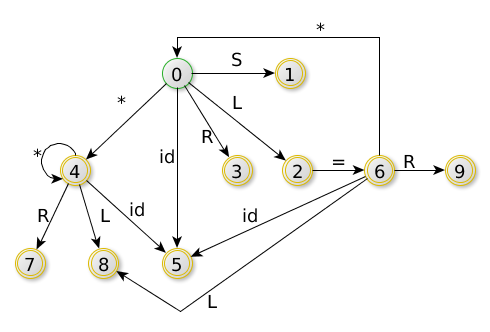
\includegraphics[scale=0.6]{Chapters/Img/c05_05.png}\\
\end{center}

0 = 
\begin{tabular}{l}
	$S' \rightarrow .S, \{ x_0 \}$\\
	$S \rightarrow .L, \{ x_0 \}$\\
	$S \rightarrow .R, \{ x_0 \}$\\
	$L \rightarrow .*R, \{ x_0 \}$\\
	$L \rightarrow .id, \{ x_0 \}$\\
	$R \rightarrow .L, \{ x_0 \}$\\
\end{tabular}\\[5pt]

1 = 
\begin{tabular}{l}
	$S' \rightarrow S., \{ x_1 \}$\\
\end{tabular}\\[5pt]

2 = 
\begin{tabular}{l}
	$S \rightarrow L. = R, \{ x_2 \}$\\
	$R \rightarrow L., \{ x_3 \}$\\
\end{tabular}\\[5pt]

3 = 
\begin{tabular}{l}
	$S \rightarrow R., \{ x_4 \}$\\
\end{tabular}\\[5pt]

4 = 
\begin{tabular}{l}
	$L \rightarrow *.R, \{ x_5 \}$\\
\end{tabular}\\[5pt]

5 = 
\begin{tabular}{l}
	$L \rightarrow id., \{ x_6 \}$\\
\end{tabular}\\[5pt]

6 = 
\begin{tabular}{l}
	$S \rightarrow L = .R, \{ x_7 \}$\\
	$R \rightarrow .L, \{ x_7 \}$\\
	$L \rightarrow .*R, \{ x_7 \}$\\
	$L \rightarrow .id, \{ x_7 \}$\\
\end{tabular}\\[5pt]

7 = 
\begin{tabular}{l}
	$L \rightarrow *R., \{ x_8 \}$\\
\end{tabular}\\[5pt]

8 = 
\begin{tabular}{l}
	$R \rightarrow L., \{ x_9 \}$\\
\end{tabular}\\[5pt]

9 = 
\begin{tabular}{l}
	$S \rightarrow L = R., \{ x_10 \}$\\
\end{tabular}\\[5pt]

$x_0 = \{ \$ \}$ \\
$x_1 = \{ x_0 \}$ \\
$x_2 = \{ x_0 \}$ \\
$x_3 = \{ x_0 \}$ \\
$x_4 = \{ x_0 \}$ \\
$x_5 = \{ \{ =, x_0 \} \cup \{ x_5 \} \cup \{ x_7 \} \}$  \\
$x_6 = \{ x_5 \}$ \\
$x_7 = \{ x_2 \}$ \\
$x_8 = \{ x_5 \}$ \\
$x_9 = \{ \{x_5\} \cup \{ x_7\} \}$ \\
$x_10 = \{ x_7 \}$ \\

Ora devo risolvere il sistema 
\begin{tabular}{ll}
		& 	\textbf{class} 	\\
	$x_0 = \{ \$ \}$	&	$x_0$ \\
	$x_1 $				&	$x_0$ \\
	$x_2 $				&	$x_0$ \\
	$x_3 $				&	$x_0$ \\
	$x_4 $				&	$x_0$ \\
	$x_5 = \{ =, x_0, x_5, x_7 \}$		&	$x_5$ \\
	$x_6 = \{ =, x_0, x_5, x_7 \}$		&	$x_6$ \\
	$x_7 $				&	$x_0$ \\
	$x_8 $				&	$x_5$ \\
	$x_9 = \{ x_5, x_7 \}$	&	$x_9$ \\
	$x_10$				&	$x_10$ \\
\end{tabular}

Mi rimangono quindi solo 4 variabili $x_0, x_5, x_6, x_9$
\begin{tabular}{ll} 
	$x_0 = \{ \$ \}$ 					& 	\\
	$x_5 = \{ =, x_0, x_5, x_7\$ \}$	& 	$= \{ =, x_0 \}$\\
	$x_6 = \{ =, x_0, x_5, x_7\$ \}$	& 	$= \{ =, x_0, x_5 \}$\\
	$x_9 = \{ x_5, x_7\$ \}$	& 	$= \{ x_5, x_0 \}$\\
\end{tabular}

Creo un grafo mettendo sui nodi le variabili, con solamente i terminali di quella variablie (non quelli presi dalle altre. Solo quelli che non sono $x_k$ insomma).

\begin{center}
    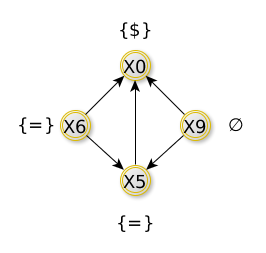
\includegraphics[scale=0.6]{Chapters/Img/c05_06.png}\\
\end{center}

Ottengo:
$x_0 = \{ \$ \}$ \\
$x_5 = \{ =, \$ \}$ \\
$x_6 = \{ =, \$ \}$ \\
$x_9 = \{ =, \$ \}$ \\

Questi sono il lookahead set che stavo cercando.

\begin{center}
    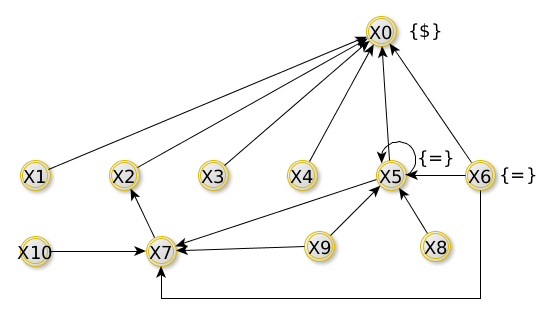
\includegraphics[scale=0.6]{Chapters/Img/c05_07.png}\\
\end{center}

\section{Costruzione automa simbolico}
\begin{lstlisting}
	x_0 = new Var();
	Vars = {x_0};
	P_0 =  closure1({[S' -> .S, {x_0}]});
	States = {P_0};
	P_0 unmarked;
	while(exists unmarked state P in States){
		mark P;
		foreach(Y in V){
			tmp = emptySet;
			foreach([A -> alpha . Y beta, delta] in P){
				tmp.Add(([A -> alpha . Y beta, delta]);
			}
			if(tmp is not empty){
				if(lo stato target non e'' ancora stato collezionato){
					States.Add(versione simbolica del target);
					Queue.Add(equazione per kernel item in tmp);
				} else {
					raffinare le equazioni delle variabili associate ai kernel item del target;
				}
			}
		}
	}
\end{lstlisting}

\section{Grammatiche Attribuite}

\begin{center}
	\begin{tabular}{ll}
		\textbf{SDD} & Syntax Directed Definition\\
		\textbf{SDT} & Syntax Directed Translation \\
	\end{tabular}
\end{center}

Una grammatica attribuita \'e una grammatica a cui sono aggiunti attributi e regole.\\[5pt]
$E \rightarrow E + T | T$\\
$T \rightarrow T * F | F$\\
$F \rightarrow (E) | id$\\
$w = 3+4*5$\

\begin{center}
    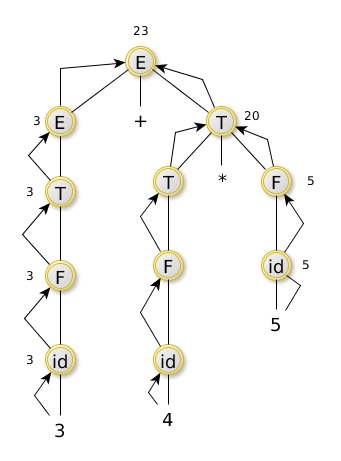
\includegraphics[scale=0.6]{Chapters/Img/c05_08.png}\\
\end{center}

Il valore di propaga dal basso verso l'alto nell'albero e computate le operazioni man mano che si presentano.\\[5pt]

\begin{tabular}{ll}
	$E_1 \rightarrow E_2 + T $ 		& 	$\{ E_1.val = E_2.val + T.val \}$	\\
	$E \rightarrow T $ 				& 	$\{ E.val = T.val \}$	\\
	$T_1 \rightarrow T_2 * F $ 		& 	$\{ T_1.val = T_2.val * F.val \}$	\\
	$T \rightarrow F $		 		& 	$\{ T.val = F.val \}$	\\
	$F \rightarrow E $		 		& 	$\{ F.valE = E.val \}$	\\
	$F \rightarrow id $ 			& 	$\{ F.val = lexval(id) \}$	\\
\end{tabular}
$\leftarrow$ Azione semantica \\[5pt]

L'abstract syntax tree di questa grammatica \'e:

\begin{center}
    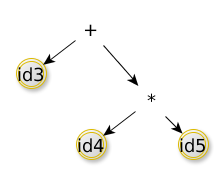
\includegraphics[scale=0.6]{Chapters/Img/c05_09.png}\\
\end{center}

\section{Attributi Sintetizzati ed Ereditati}
$A \rightarrow \alpha$ A.a definito come una funzione degli attributi dei terminali e non terminali in $\alpha$. Gli attributi dei terminali sono informazioni ottenute 
durante l'analisi lessicale.

\subsection{Esempio}
\begin{tabular}{ll}
	$D \rightarrow TL$ 			&	$ \{ L.i = T.t \} $\\
	$T \rightarrow int$ 		&	$ \{ T.t = integer \} $\\
	$T \rightarrow float $ 		&	$ \{ T.t = float \} $\\
	$L_1 \rightarrow L_2,\ id$ 	&	$ \{ L_2.i = L_1.i; addType(lexval(id), L_1.i) \} $\\
	$L \rightarrow id$ 			&	$ \{ addType(lexval(id), L_i) \} $\\
\end{tabular}

w = int pluto, pippo, paperino 

\begin{center}
    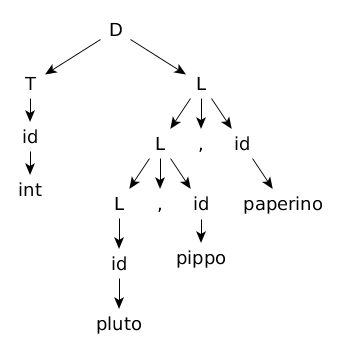
\includegraphics[scale=0.6]{Chapters/Img/c05_10.png}\\
\end{center}

Facendo bottom-up la prima cosa che faremo sar\'a $T \rightarrow int$. A questo punto T conosce \lq\lq int\rq\rq\ e lo dice alla L pi\'u in alto (quella subito sotto a D).
Quella L lo dice alla L sotto di lui, e questo succede anche per il livello dopo. Adesso L va ad \lq\lq id\rq\rq\ che diventa \lq\lq pluto\rq\rq\, che L viene a conoscere
(poich\'e viene passato in alto). Visto che alcuni attributi dipendono dai padri e dagli attributi dei fratelli, questi sono attributi ereditati.

Gli attributi ereditati sono funzione degli attributi di siblings e del padre.

\subsection{Esempio}
$S \rightarrow N$\\
$N \rightarrow o\ Digist$\\
$N \rightarrow Digits$\\
$Digits \rightarrow Digits\ d$\\
$Digits \rightarrow d$\\

Questo albero \'e simile a quello di prima: c\'e solo \lq\lq o\rq\rq\ a sinistra e potenzialmente infinite \lq\lq Digits\rq\rq\ a destra, una sotto l'altra.
Come fare per essere in grado di distinguere se c\'e la \lq\lq o\rq\rq\ oppure no?

Posso ribaltare l'albero, riscrivendo la grammatica come:\\
\begin{tabular}{ll}
	$S \rightarrow Digits$ 	&	$\{ Digits.qualcosa \}$\\
	$Digits_1 \rightarrow Digits_2 \ d $ 	&	$\{ Digits_1.val = Digits_2.val * Digits_2.base + 'd' \}$\\
	$Digits \rightarrow d $ 	&	$\{ Digits.base = 8;\ Digits.val = 'd' \}$\\
	$Digits \rightarrow od $ 	&	$\{ Digits.base = 10;\ Digits.val = 'd' \}$\\
\end{tabular}
